%% Copernicus Publications Manuscript Preparation Template for LaTeX Submissions
%% ---------------------------------
%% This template should be used for copernicus.cls
%% The class file and some style files are bundled in the Copernicus Latex Package which can be downloaded from the different journal webpages.
%% For further assistance please contact the Copernicus Publications at: publications@copernicus.org
%% http://publications.copernicus.org


%% Please use the following documentclass and Journal Abbreviations for Discussion Papers and Final Revised Papers.


%% 2-Column Papers and Discussion Papers
%\documentclass[gmd, manuscript]{copernicus}
\documentclass[gmd]{copernicus}



%% Journal Abbreviations (Please use the same for Discussion Papers and Final Revised Papers)

% Geoscientific Model Development (gmd)
% Hydrology and Earth System Sciences (hess)




%% \usepackage commands included in the copernicus.cls:
%\usepackage[german, english]{babel}
%\usepackage{tabularx}
%\usepackage{cancel}
%\usepackage{multirow}
%\usepackage{supertabular}
%\usepackage{algorithmic}
%\usepackage{algorithm}
%\usepackage{float}
%\usepackage{subfig}
%\usepackage{rotating}


\begin{document}

\linenumbers

\title{AtmoSwing (v1.4): Analog Technique Model for Statistical weather forecastING}


% \Author[affil]{given_name}{surname}

\Author[1,2]{Pascal}{Horton}
\Author[1]{Michel}{Jaboyedoff}
\Author[3]{Charles}{Obled}

\affil[1]{University of Lausanne, Lausanne, Switzerland}
\affil[2]{Terranum, Lausanne, Switzerland}
\affil[3]{Universit\'{e} de Grenoble-Alpes, LTHE, Grenoble, France}

%% The [] brackets identify the author with the corresponding affiliation. 1, 2, 3, etc. should be inserted.



\runningtitle{AtmoSwing}

\runningauthor{P. Horton et al.}

\correspondence{Pascal Horton (pascal.horton@alumnil.unil.ch)}



\received{}
\pubdiscuss{} %% only important for two-stage journals
\revised{}
\accepted{}
\published{}

%% These dates will be inserted by Copernicus Publications during the typesetting process.


\firstpage{1}

\maketitle



\begin{abstract}

The analogue method allows forecasting local meteorological variables of interest (predictand), such as the daily precipitation, on the basis of synoptic variables (predictors). It relies on the fact that similar meteorological influences are likely to result in similar local effects. This statistical relationship is thus based on archives of observed data, and used in order to operationally forecast the coming days, or to evaluate future conditions under a changing climate.

AtmoSwing is an open source software that implement the analogue method in a very flexible way, so that different variants can be handled dynamically, by parameterization trough XML files. It is made of 3 tools: the Forecaster to perform operational forecasts, the Viewer to display the results, and the Optimizer to establish the statistical relationship between the predictand and predictors. 

The Forecaster handles every required step internally, such as predictors downloading and parsing, grid interpolation, analogy sorting, without external scripts or file conversion. The processing of a forecast is extremely lightweight in terms of IT infrastructure; it can indeed run on almost any computer.

The Viewer displays the forecasts in an interactive GIS environment. It contains several layers of syntheses and details in order to provide a quick overview of the potential critical situations in the coming days, as well as the possibility for the user to go into the details of the forecasted predictand and criteria distributions. Several tips coming from the literature are provided in order to help interpreting the forecasts.

The Optimizer integrates the most used technique, that is a semi-automatic sequential approach, as well as Monte-Carlo analyses, and a global optimization technique by means of Genetic algorithms. It allows establishing the statistical relationship between predictors and predictands. 


\end{abstract}



\introduction  %% \introduction[modified heading if necessary]

Reasoning by analogy is rather widespread in different domains of sciences or engineering. In hydrometeorology, it consists, given a certain situation, in looking into the past to retrieve situations that can be considered similar and therefore with consequences that may be expected similar to the situation at hand. By situation, we often think of the atmospheric situation over a rather wide domain, but it may also be the atmospheric profile at a radio-sounding station or the air-snow state at a given mountain observing station. By consequence, we often focus on one (or more) local variable of interest, such as the occurrence of hail, storm, avalanches, or the amount of wind or precipitation over a given region.

As a general setting, the required ingredient are a couple of archives, one describing the situation through different variables, called predictors, and another one giving, for those situations, the value of the local variable of interest for engineering purpose, called predictand.  Obviously, one understands that the longest and the richest the candidate archive of predictors, the more chance there will be to extract good analogues for a target situation in order to derive a conditional range of predictand values. As for the predictors, we can now hopefully rely on rich reanalysis products, commonly available over 40 years or more, and easily accessible. 

Usually, the predictand values could be derived in a rather physical-dynamic approach  by modeling the chain of processes linking the predictors to the predictand. However, the model may be extremely complex, time consuming, or some processes may be poorly known or parameterised. Conversely, the hope is that given the past archive of predictors, enough situations analogues to a target one could be found so that reasonable values will be found for the predictand, at a reasonable coding and computing-time costs. This is particularly true for a predictand much required in hydrometeorological applications, namely the precipitation amount over a given domain and time duration. The processes involved range from large scale dynamical states of the atmosphere down to very small scale microphysical processes, requiring models that are extremely complex, data-demanding, and time consuming. Therefore, with an appropriate set of archives, one may bypass all these modeling aspects by obtaining the predictand values observed from past analogue situations.

The purpose of this paper is not to argue in favour or against this approach, which has proved to be used efficiently either in operational forecasting or more recently in climate studies, and which is capable of challenging more classical approaches based on meteorological modeling. In operational forecasting, it has been used mainly by practitioners, notably hydropower companies or flood forecasting services, while in climate studies, it is more and more used to downscale the results of global climate model simulation runs. In operational, it should however not to be considered as a substitution for numerical weather prediction models, but as a complement in order to get a fast and independent forecast that is known to be accurate several days in advance. It therefore enriches the analysis of a potential critical situation for flood forecasting, for example, and is very interesting in early warning.

However, how efficient and useful it may seem, this approach is not straightforward. Usually the type of predictand is imposed by some practical needs or constraints. Considering a precipitation variable, ones has to decide upon the duration of accumulation, (e.g. from 6-hourly to daily or several day totals) according for example to the size or response time of a the catchments to be managed. We must also consider the availability and quality of a long enough time series. Moreover, the analogy is restricted to a selection of variables at a specific time and over optimized spatial domains, that are compared by means of a chosen criteria that can rank the candidate days from the archive with a distance quantification. The approach appears predictand-specific but also dependent on the archive of predictors. Thus, the analogy is defined by many parameters (choice of the predictor variable, the temporal and spatial windows, and the number of analogues to consider) that are not straightforward to determine. 

We will first present the AM along with various implementations, as the optimal version of the method may vary with the location of interest, and as all these can be processed with AtmoSwing. The software will then be presented, and its modules detailed, such as the Forecaster and the Viewer that are tools for operational use, and the Optimizer that allows optimizing the method for a given predictand time series.



\section{The analogue method}

As AtmoSwing does not rely heavily on one variant of the analogue method (AM), but can implement different parametrization, we gathered here several references of possible implementations as well as the main evolution steps of the AM. This latter summarizes the improvements that were brought, as well as discontinued approaches that were found less relevant (such as the use of PCA on the predictors).

\subsection{Principles}

The AM is based on the principle that two similar synoptic situations may produce similar local effects \citep{Lorenz1956}. The perfect analogy does not exist, but sufficiently similar situations leading to similar effects can be identified. Thus, two states of the atmosphere that are alike are called analogues \citep{Lorenz1969}. To be relevant, this analogy must be selected by optimizing the following elements:

\begin{itemize}
	\item The analogy variable (the predictor) must contain synoptic information having indirect dependency with the local weather and the target variable (often the precipitation).
	\item The spatial window is the domain on which the analogy variable is considered. The ideal size of this area is one that maximizes useful information.
	\item The temporal window is the hour of day at which we consider the analogy variable. The analogy can be instantaneous (eg. 12~h~UTC) or averaged over a period (eg. 24~h).
	\item The analogy period is the time of year in which similar situations are being sought. Thus, we compare situations with a similar distribution of solar energy \citep{Lorenz1969}.
	\item The analogy criterion, needed to compare the variables on the chosen spatial and temporal windows, is a score used for ranking past situations according to their degree of similarity with the target situation \citep{Bontron2004}.
	\item The ideal number of analogues situations is the best compromise in order to take into account local variability and to maximize useful synoptic information  \citep{Bontron2004}.
\end{itemize}

Because of the chaotic nature of the atmosphere, two analogue situations quickly diverge over time \citep{Lorenz1969}. Thus, the AM has strong limitations regarding the temporal extrapolation \citep{Bontron2004}. Numerical models being more capable of simulating the dynamic evolution of the atmosphere, the temporal extrapolation of the synoptic variables is left to them. The search for analogy aims thus at connecting the forecasted synoptic situation with a local predictand (temperature, precipitation ...), which is more difficult to simulate by numerical models.

The AM is being used for many years at EDF (\'{E}lectricit\'{e} de France), to build precipitation and temperature scenarios \citep{Desaint2008a}. It is also operational at the Compagnie Nationale du Rh\^{o}ne (CNR, France) and some flood forecasting services (SPC) in France and Switzerland \citep{Marty2010,GarciaHernandez2009b,Horton2012}.


\subsection{Data}
\label{sec:data}

The AM relies on two types of data: predictors, that are atmospheric variables describing the state of the atmosphere at a synoptic scale, and the predictand, which is the local weather time series we want to forecast.

Predictors are generally reanalysis datasets (as archive) and outputs of a global numerical weather prediction models for the target situation in operational forecasting. Reanalysis datasets, such as the NCEP/NCAR reanalysis I \citep[6-hourly, 17 pressure levels at a resolution of 2.5\degree, see][]{Kalnay1996}, the NCEP/DOE reanalysis II \citep{Kanamitsu2002}, ERA-40 \citep{Uppala2005} are often used and can be inputed in AtmoSwing. Other observed predictors can also be used, such as Sea Surface Temperature \citep[SST, ][]{Reynolds2007}. The predictors describing the target situation in operational forecasting can for example result from GFS \citep[Global Forecast System,][]{Kanamitsu1991,Kanamitsu1989}, which is operated by NCEP and NOAA.

\citet{Bontron2004} determined that the length of the archive should be 30 years to forecast usual situations, and 40 years for intense events. He also highlighted the dependence between the optimal number of analogues and the archive size: the shorter the archive, the lower the number of analogues. By varying the resolution of the predictors grids, he concluded that the performance increase is not significant for the analogy of atmospheric circulation below a resolution of 5\textdegree. However, it seems more important for the second level of analogy on moisture, which are more local variables. \citet{BenDaoud2010} assessed the European reanalysis ERA-40 \citep{Uppala2005} with a resolution of 1.125\textdegree. He identified a slight performance improvement, but not substantial enough to really justify an archive change \citep{BenDaoud2008}.

The predictand is the local meteorological variable of interest. It can be 6-houry data, or more often daily time series, but has to be consistent with the time step of the predictors (at least, not finer). The most used predictor is the daily precipitation, usually averaged over subregions in order to smooth local effects \citep{Obled2002, Marty2012}. These time series are frequently normalized by the precipitation value for a return period of 10~years \citep{Djerboua2001}. This normalization allows for an easier comparison between subregions subject to different precipitation regimes, and thus to better identify the most important contributions. Most users also apply a root square to this last ratio in order to reduce the weight of the extreme predictand values, but we generally don't.


\subsection{Present structure}

Although multiple variations of the AM exist, they generally share the same basics and the same structure. We want here to forecast the daily precipitation (the predictand) for a target day (at a defined lead time) and have long archives of both the predictand and predictor variables. The generic structure is the following:

\begin{enumerate}
	\item Preselection: to cope with seasonal effects, candidate dates are extracted from the archive within a period of four months centered around the target date, for every year of the archive. Alternatively, the candidate dates can be selected based on similar air temperature \citep{BenDaoud2010}.
	
	\item First level of analogy: we subsample $N_{1}$ dates within all the candidates provided by the preselection, by means of an analogy ranking. The first level of analogy is always the atmospheric circulation when it comes to precipitation forecasting. We thus assess the similarity of the atmospheric circulation of our target date with all the situations provided by the preselection by means of the S1 criteria \citep[Eq.\ref{eq:S1}, ][see also section \ref{sec:method:evolution}]{Teweles1954, Drosdowsky2003}, which is a comparison of gradients, over a certain spatial window.
	
	\begin{equation}
	\label{eq:S1}
	S1=100 \frac {\displaystyle \sum_{i} \vert \Delta\hat{z}_{i} - \Delta z_{i} \vert}
	{\displaystyle \sum_{i} max\left\lbrace \vert \Delta\hat{z}_{i} \vert , \vert \Delta z_{i} \vert \right\rbrace }
	\end{equation}
	where $\Delta \hat{z}_{i}$ is the forecast geopotential height difference between the \textit{i}th pair of adjacent points in the target situation, and $\Delta z_{i}$ is the corresponding observed geopotential height difference in the candidate situation. The differences are processed separately in both directions. The smaller the S1 values are, the more similar the pressure fields.
	
	The $N_{1}$ dates with the lowest values of S1 are considered as analogues to the target day. The number of analogues, $N_{1}$, is a parameter to calibrate.
	
	\item Subsequent level(s) of analogy: we can then subsample once again the $N_{1}$ analogues on the basis of another variable in order to obtain a lower number of analogue dates, $N_{2}$. The S1 criterion is usually not relevant for other predictors that the atmospheric circulation. Other classic criteria represent absolute distances: Mean Absolute Error (MAE) and Root Mean Squared Error (RMSE), the latest being most often used. These are more relevant to compare moisture variables for example.
	
	This process can be repeated, by subsampling a decreasing number of analogues, $N_{i}$, according to a ranking processed on various meteorological variables.
	
	\item Probabilistic forecast: then, the daily observed precipitation amount (or another predictand of interest) of the $N_{i}$ resulting dates provide the empirical conditional distribution considered as the probabilistic forecast for the target day. The empirical frequencies are processed for every value of the predictand, after classification, based on the Gringorten parameters (for a Gumbel or exponential law).
	
\end{enumerate}


\subsection{Proposed nomenclature}

Variants of the AM parameterization are numerous and it is not always easy to reference them in a short and descriptive way. We thus propose a basic nomenclature (Figure \ref{figure:nomenclature}) in order to give an idea of the structure in a simple identifier. This one cannot describe all the parameters of the AM, but quickly illustrate the structure of the implementation. This is particularly useful when working with a global optimization method, where nothing is fixed but the very structure of the AM.

\begin{figure}[htbp]
	\includegraphics[width=8.3cm]{figures/nomenclature.pdf}
	\caption{Proposed structure for naming the parameterizations of the AM.}
	\label{figure:nomenclature}
\end{figure}

The naming contains different blocs (separated by an hyphen) for the various levels of analogy. It starts with the specification of the preselection (P; can be omitted when comparing AMs with the same preselection approaches), which can be nowadays of 2 types:
\begin{itemize}
	\setlength\itemsep{-2px}
	\item C: calendar period ($\pm 60$ days around the target date)
	\item T: based on air temperature \citep{BenDaoud2010}
\end{itemize}

Then, the following levels of analogy are listed. They may start with an optional A (for analogy) when other methods are mixed into the parameterization \citep[see eg. ][]{Chardon2014}. For every level of analogy, we first provide the number of variables used (combination of atmospheric levels and time of observation) and then give the short name of the variable (according eg to ECMWF conventions; in upper case), for example:
\begin{itemize}
	\setlength\itemsep{-2px}
	\item Z : geopotential (circulation)
	\item MI : moisture index (TPW * RH)
	\item MF : moisture flux (V * TPW * RH)
	\item TPW : total precipitable water
	\item V : wind velocity
	\item W : vertical velocity
\end{itemize}

In order to keep the identifier simple, no value of atmospheric level neither time of observation is specified. Moreover, the analogy criterion is not specified and is supposed to be S1 for Z and RMSE for the other variables. If anything changes from these conventions, it can be noted as a flag. The flag (lower case) can also give other information, such as the optimization method:
\begin{itemize}
	\setlength\itemsep{-2px}
	\item sc : sequential calibration (can be omitted as considered as default, see section \ref{sec:atmoswing-calibration})
	\item go : global optimization (by means of genetic algorithms for example)
\end{itemize}

This nomenclature can be adapted to specific needs, or simplified for a better readability (eg. by removing the specification of the preselection). Examples are provided in the following section.


\subsection{Evolution of the method for precipitation forecasting}
\label{sec:method:evolution}

The evolution of the AM for precipitation forecasting led to several improvements. However, some of these are specific for a certain region and are not relevant for others, and some perform better depending on the lead time. Thereby, we cannot provide a single best parameterization for the AM, neither rank them from worst to best. We will thus provide some examples of parameterizations of the most recent AM variant, in the chronological order they appeared. The most common usage of the AM is for precipitation forecasting. Thus, the evolution presented hereafter focuses on this predictand. However, the AM, or an equivalent, was also used for short to medium term forecasting of daily temperatures \citep{Radinovic1975, Woodcock1980, Kruizinga1983}, wind \citep{Gordon1987}, snow avalanches \citep{Obled1980, Bolognesi1993}, insolation \citep{Bois1981}, and the trajectory of tropical cyclones \citep{Keenan1981, Sievers2000, Fraedrich2003}. \citet{Guilbaud1997} performed a literature review about the use of the AM in long-term forecasting and identified operational applications for monthly forecasts in many countries, including Canada \citep{Shabbar1986},  Hungary \citep{Toth1989}, the Netherlands \citep{Nap1981}, and England \citep{Murray1974}, as well as seasonal forecasts: \citet{Barnett1978}, \citet{Bergen1982} and \citet{Livezey1988}.

\citet{Lorenz1969} introduced the concept and established the basis of the AM. He considered looking for analogues on the geopotential field (at 200, 500 and 850~hPa) with a corrected Euclidean distance averaged on the 3 levels. In addition, the analogue situations were to belong to the same period of the year to be comparable in terms of distribution of solar energy.

The use of the AM for operational forecasting of daily precipitation originates in the work of \citet{Duband1970, Duband1974, Duband1981}. It was then designed for operational forecasting at EDF (\'{E}lectricit\'{e} de France) in order to better manage water resources and flood risks. The geopotential height at 700~hPa and 00~h was used for its higher stability than the sea level pressure (SLP) field, and its sensitivity to the atmospheric disturbances \citep{Guilbaud1997}. However, the SLP at 06~h was also used for determining the intensity of precipitation, as well as the temperature at 700~hPa as indicator of the thermal state of the air mass \citep{Duband1974}. The data were then based on 37 radiosounding over Europe and condensed by a principal component analysis. The first 25 analogues on the geopotential at 700~hPa were considered, and multiple local regressions between precipitation, SLP, and the temperature at 700~hPa were established on these analogues before being applied to the target situation \citep{Guilbaud1997}. The archives were split by season to consider comparable situations in terms of distribution of solar energy \citep{Lorenz1969}. This initial rigid division into seasons was then transformed into a moving selection of more or less two months around the target date. The forecast was then performed only on the basis of observations and was temporally extrapolated to the following two days. After a few years, this statistical temporal extrapolation was abandoned in favor of a statistical adaptation using predictors resulting from an global numerical model, allowing a forecast over the following 4~days.

Thereafter, the geopotential was considered at 1000~hPa and 700~hPa and the analogues selection was done in two stages: first according to an Euclidean distance in the space of the principal components of the geopotential field at 700~hPa, and then according to a correlation criterion (on the geopotential field at 700 and 1000~hPa, as well as on the thickness between these two levels) in order to remove days too dissimilar \citep{Guilbaud1997}. The regression approach to determining precipitation was eventually abandoned in favor of the probabilistic forecasting (synthesized by the percentiles 20, 60 and 90~\%), as it is performed today by interpolating linearly over the cumulative empirical distribution of daily precipitation measured at the analogue days \citep{Guilbaud1997, Guilbaud1998}.

\citet{Wilson1980} sought the 20 best analogues on the geopotential field at 500 and 1000~hPa using the Teweles-Wobus (S1) criterion (Eq. \ref{eq:S1}), which allows for a comparison of the gradients and thus an analogy of the atmospheric circulation. \citet{Woodcock1980} used the same criterion on the SLP fields to select 50~analogues in order to forecast maximum daily temperatures. \citet{Yacowar1975} considered the 20 best analogues on the maximum of the sum of correlations on the two fields. This work has demonstrated the best performance of the AM compared to regression methods, as well as the interest to search for analogues on two (500 and 1000~hPa) geopotential fields combined \citep{Guilbaud1997}.

\citet{Mandon1985} introduced a second level of analogy and assessed different variables, such as wind, moisture, air temperature, surface temperature of the Mediterranean, the product of wind and the 700~hPa moisture, as well as a second barometric criteria differentiated according to the season. \citet{Vallee1986} continued to work on the second level of analogy and considered the wind at 700~hPa \& 12~h in order to improve heavy precipitation events for a region in France susceptible to southerly flows.

Taking advantage of higher-performance IT tools \citet{Guilbaud1997} stopped using PCA in order to work directly with the raw data interpolated on grids, which was an improvement, especially when considering the S1 criterion (already used for analogues selection by\citealp{Wilson1980} and \citealp{Woodcock1980}) instead of the Euclidean distance. This score gives importance to the similarity of atmospheric circulation rather than absolute values of the pressure field. After comparing this criterion to other criteria from the literature, or combinations of these, \citet{Guilbaud1998} found that S1 is the most efficient. They also pointed out the benefit of using 2 atmospheric levels, 1000~hPa (Z1000) and 700~hPa (Z700) or 500~hPa (Z500), instead of one (also instead of the thickness), and to also consider 2 temporal windows, 00~h and 24~h \citep{Obled2002}. The number of analogues considered is 50 (Table \ref{table:R0}). When using multiple predictors, they combined the criteria values calculated on each atmospheric level and each temporal window using an arithmetic mean. Finally, they also suggested using a second level of analogy on lower layers moisture and introduced the Ranked Probability Score \citep{Epstein1969} to assess the forecast quality, which was found to be more relevant that the Brier score \citep{Brier1950}.

\begin{table}[htbp]
	\caption{Method of type PC-4Z proposed by \citet{Guilbaud1997}.}
	\begin{tabular}{ccccc}
		\tophline
		\textbf{Level} & \textbf{Variable} & \textbf{Hour} & \textbf{Criteria} & \textbf{Nb} \\ 
		\middlehline
		0 & \multicolumn{4}{l}{$\pm 60$ days around the target date} \\
		\middlehline 
		\multirow{2}{*}{1} & Z1000 & 00, 24~h & \multirow{2}{*}{S1} & \multirow{2}{*}{50} \\
		& Z700 $^{\dagger}$ & 00, 24~h & & \\ 
		\bottomhline 
	\end{tabular} 
	\belowtable{$\dagger$ or Z500 as an alternative}
	\label{table:R0}
\end{table}

\citet{Bontron2004} could benefit from the newly available NCEP/NCAR reanalysis data. This dataset being more homogeneous, much longer, and contained more variables than what was previously used, he could systematically assess a large selection of variables in the AM combined with different criteria. He thus confirmed the interest of the geopotential height along with the S1 criterion for the first level of analogy. He has also shown that the choice of the temporal window (time of observation) has a higher importance than the atmospheric level for the performance of the AM. By assessing multiple combinations of atmospheric levels and temporal windows, he concluded that the coupled geopotential heights at 1000~hPa (Z1000) \& 12~h and 500~hPa (Z500) \& 24~h provided the best performance for the studied region (Table \ref{table:R1}). The analogy on the atmospheric circulation proposed by \citet{Bontron2004} is still, at the time of writing, often used operationally, and considered as a reference for benchmarking new parameterizations \citep{Horton2012, BenDaoud2015}.

\begin{table}[htbp]
	\caption{Method of type PC-2Z proposed by \citet{Bontron2004}.}
	\begin{tabular}{ccccc}
		\tophline
		\textbf{Level} & \textbf{Variable} & \textbf{Hour} & \textbf{Criteria} & \textbf{Nb} \\ 
		\middlehline 
		0 & \multicolumn{4}{l}{$\pm 60$ days around the target date} \\
		\middlehline 
		\multirow{2}{*}{1} & Z1000 & 12~h & \multirow{2}{*}{S1} & \multirow{2}{*}{50} \\
		& Z500 & 24~h & & \\ 
		\bottomhline 
	\end{tabular} 
	\label{table:R1}
\end{table}

\citep{Bontron2004} also assessed several variables for the second level of analogy and identified the moisture variables (precipitable water and relative humidity) and vertical velocity to be the most relevant. Finally, he found that a moisture index made of the product of relative humidity at 850~hPa (RH850) and total precipitable water (TPW) gave the best performance (Table \ref{table:R2}). This index does not represent an actual physical quantity, but expresses the water content of the column and its proximity to saturation.

\begin{table}[htbp]
	\caption{Method of type PC-2Z-2MI proposed by \citet{Bontron2004}.}
	\begin{tabular}{ccccc}
		\tophline
		\textbf{Level} & \textbf{Variable} & \textbf{Hour} & \textbf{Criteria} & \textbf{Nb} \\ 
		\middlehline 
		0 & \multicolumn{4}{l}{$\pm 60$ days around the target date} \\
		\middlehline 
		\multirow{2}{*}{1} & Z1000 & 12~h & \multirow{2}{*}{S1} & \multirow{2}{*}{70} \\
		& Z500 & 24~h & & \\ 
		\middlehline
		2 & TPW * RH850 & 12, 24~h & RMSE & 30 \\
		\bottomhline 
	\end{tabular} 
	\label{table:R2}
\end{table}

He noted the relevance of defining different spatial windows for each region, rather than a single window to the entire territory. These windows are more able to represent the specific atmospheric influences for the region. In order to assess the forecast, he introduced the Continuous Ranked Probability Score \citep[CRPS, Eq. \ref{eq:CRPS}, ][]{Brown1974}, which discards the issue of determining classes as with the RPS previously in use.

\citet{Gibergans-Baguena2007} implemented the AM for daily precipitation forecasts in Catalonia. They considered the geopotential at 700 and 1000~hPa, and the thickness between these two levels, to search for analogy of circulation, and then applied a second selection on local data from radiosonde: stability indexes, precipitable water, temperature, etc.

\citet{Marty2010} tested other temporal windows for intraday application on the basis of a more comprehensive reanalysis dataset. He first proposed to change the hours of observation for both levels of analogy (both for 06~h and 18~h), and selected the 925~hPa level for the moisture analogy (Table \ref{table:R3a}). The selected hours and atmospheric levels were not available before.

\begin{table}[htbp]
	\caption{Method of type PC-2Z-2MI proposed by \citet{Marty2010}.}
	\begin{tabular}{ccccc}
		\tophline
		\textbf{Level} & \textbf{Variable} & \textbf{Hour} & \textbf{Criteria} & \textbf{Nb} \\ 
		\middlehline 
		0 & \multicolumn{4}{l}{$\pm 60$ days around the target date} \\
		\middlehline 
		\multirow{2}{*}{1} & Z1000 & 06~h & \multirow{2}{*}{S1} & \multirow{2}{*}{75} \\
		& Z500 & 18~h & & \\ 
		\middlehline
		2 & TPW * RH925 & 06, 18~h & RMSE & 30 \\
		\bottomhline 
	\end{tabular} 
	\label{table:R3a}
\end{table}

Then, \citet{Marty2010} changed the moisture index into the moisture flux by adding the wind velocity (V700 or V925) component in the multiplication. He considered this flux at 700~hPa or 925~hPa (Table \ref{table:R3b}).

\begin{table}[htbp]
	\caption{Method of type PC-2Z-2MF proposed by \citet{Marty2010}.}
	\begin{tabular}{ccccc}
		\tophline
		\textbf{Level} & \textbf{Variable} & \textbf{Hour} & \textbf{Criteria} & \textbf{Nb} \\ 
		\middlehline 
		0 & \multicolumn{4}{l}{$\pm 60$ days around the target date} \\
		\middlehline 
		\multirow{2}{*}{1} & Z1000 & 06~h & \multirow{2}{*}{S1} & \multirow{2}{*}{60} \\
		& Z500 & 18~h & & \\ 
		\middlehline
		2 & V700 * TPW * RH700 $^{\dagger}$ & 06, 18~h & RMSE & 25 \\
		\bottomhline 
	\end{tabular} 
	\belowtable{$\dagger$ or V925 * TPW * RH925 as an alternative}
	\label{table:R3b}
\end{table}

\citet{BenDaoud2010} applied the AM in the context of large floodplains, out of an Alpine environment (Sa\^{o}ne, Seine). He evaluated several variables usually used in weather forecasting, amongst them the air temperature and the vertical velocity that presented a potential interest. The temperature (at the nearest grid point, on the 925~hPa (36~h) and 600~hPa (12~h) levels) could replace the rigid calendar preselection of $\pm$ 60 days around the target date by a more dynamic screening of similar situations in terms of air masses. The seasonal effect is indeed also present in the temperature data. The number of preselected dates is equivalent to the number of days we would have chosen with the calendar approach, and thus depends on the archive size: $N_{0} = 60 \cdot 2 \cdot n_{a}$ where $n_{a}$ is the number of years in the calibration period. \citet{BenDaoud2010} also reconsidered the parameters of the moisture index and ended up with both 925~hPa and 700~hPa levels, at 12~h and 24~h, or at every time step (6~h) between 06~h and 30~h (Table \ref{table:R4b}).

\begin{table}[htbp]
	\caption{Method of type P2T-2Z-4MI (or P2T-2Z-10MI for the alternative version), by \citet{BenDaoud2010}.}
	\begin{tabular}{ccccc}
		\tophline
		\textbf{Level} & \textbf{Variable} & \textbf{Hour} & \textbf{Criteria} & \textbf{Nb} \\ 
		\middlehline
		\multirow{2}{*}{0} & T925 & 36~h & \multirow{2}{*}{RMSE} & \multirow{2}{*}{$N_{0}$} \\
		& T600 & 12~h & & \\ 
		\middlehline 
		\multirow{2}{*}{1} & Z1000 & 12~h & \multirow{2}{*}{S1} & \multirow{2}{*}{70} \\
		& Z500 & 24~h & & \\ 
		\middlehline
		\multirow{2}{*}{2} & TPW * RH925 & 12, 24~h $^{\dagger}$ & \multirow{2}{*}{RMSE} & \multirow{2}{*}{25} \\
		& TPW * RH700 & 12, 24~h $^{\dagger}$ & & \\ 
		\bottomhline 
	\end{tabular} 
	\belowtable{$\dagger$ or 06-30~h as an alternative}
	\label{table:R4b}
\end{table}

Subsequently, \citet{BenDaoud2010} added an additionally level of analogy, between the circulation and the moisture analogy (Table \ref{table:R5}), based on vertical velocity at 850~hPa (W850). This AM was developed for large plains in France, but was found to be not relevant for an Alpine environment where topography is mostly responsible for uplift of air masses \citep{Horton2012}. 

\begin{table}[htbp]
	\caption{Method of type P2T-2Z-4W-4MI, by \citet{BenDaoud2010}.}
	\begin{tabular}{ccccc}
		\tophline
		\textbf{Level} & \textbf{Variable} & \textbf{Hour} & \textbf{Criteria} & \textbf{Nb} \\ 
		\middlehline
		\multirow{2}{*}{0} & T925 (1 point) & 36~h & \multirow{2}{*}{RMSE} & \multirow{2}{*}{$N_{0}$} \\
		& T600 (1 point) & 12~h & & \\ 
		\middlehline 
		\multirow{2}{*}{1} & Z1000 & 12~h & \multirow{2}{*}{S1} & \multirow{2}{*}{170} \\
		& Z500 & 24~h & & \\ 
		\middlehline
		2 & W850 & 06-24~h & RMSE & 70 \\
		\middlehline
		\multirow{2}{*}{3} & TPW * RH925 & 12, 24~h & \multirow{2}{*}{RMSE} & \multirow{2}{*}{25} \\
		& TPW * RH700 & 12, 24~h & & \\
		\bottomhline 
	\end{tabular}
	\label{table:R5}
\end{table}

\citet{Bliefernicht2010} proposed to add a weighting to the grid points of the predictor to overcome a comparison on a fixed-size window, and to give more importance to regions with relevant atmospheric circulation information. However, he noticed that there is a risk of overparametrization and a simplification of the weighting fields may be necessary, and that the performance was not stable between the calibration and the validation periods. He also compare the performance of the AM with a forecasting method based on a weather types approach, and concluded that the AM was more efficient.

\citet{Horton2012} identified that the analogy on the atmospheric circulation may not be comprehensive, and that a significant gain was obtained by considering 4 atmospheric levels (1000, 850, 700, and 500~hPa at 12 or 24~h) instead of 2 (Table \ref{table:R6}). No number of analogues ($N_{1}$) was provided globally, as it was calibrated for every subregion. Considering a AM only based on the atmospheric circulation has an interest for operational forecasting, where moisture variables are less well forecasted over a lead time of a few days. An equivalent structure was also optimized by means of generic algorithms (PC-4Zgo), which is the topic of another paper.

\begin{table}[htbp]
	\caption{Method of type PC-4Z proposed by \citet{Horton2012}.}
	\begin{tabular}{ccccc}
		\tophline
		\textbf{Level} & \textbf{Variable} & \textbf{Hour} & \textbf{Criteria} & \textbf{Nb} \\ 
		\middlehline 
		0 & \multicolumn{4}{l}{$\pm 60$ days around the target date} \\
		\middlehline 
		\multirow{4}{*}{1} & Z1000 & 12~h & \multirow{4}{*}{S1} & \multirow{4}{*}{$N_{1}$} \\
		& Z850 & 24~h & & \\ 
		& Z700 & 12~h & & \\ 
		& Z500 & 24~h & & \\ 
		\bottomhline 
	\end{tabular}
	\label{table:R6}
\end{table}

\citet{Horton2012} also integrated an analogy on the moisture flux, after the circulation analogy on the 4 atmospheric levels (Table \ref{table:R7}). The number of analogues ($N_{1}$, $N_{2}$) were also calibrated for every subregion. Similarly, an equivalent structure was optimized (PC-4Zgo-2MIgo).

\begin{table}[htbp]
	\caption{Method of type PC-4Z-2MI, by \citet{Horton2012}.}
	\begin{tabular}{ccccc}
		\tophline
		\textbf{Level} & \textbf{Variable} & \textbf{Hour} & \textbf{Criteria} & \textbf{Nb} \\ 
		\middlehline 
		0 & \multicolumn{4}{l}{$\pm 60$ days around the target date} \\
		\middlehline 
		\multirow{4}{*}{1} & Z1000 & 12~h & \multirow{4}{*}{S1} & \multirow{4}{*}{$N_{1}$} \\
		& Z850 & 24~h & & \\ 
		& Z700 & 12~h & & \\ 
		& Z500 & 24~h & & \\ 
		\middlehline
		2 & V700 * TPW * RH700 & 12, 24~h & RMSE & $N_{2}$ \\
		\bottomhline 
	\end{tabular}
	\label{table:R7}
\end{table}

The optimal predictors vary from one region to another, along with the leading atmospheric processes. We will thus never get a unique parameterization of the AM valid for any place on earth, but the method needs to be adapted to the local conditions and to the size of the catchment of interest. Thus, there will always be local adaptations to be made for use in a new region.



% TODO : Sabine
% TODO : J�r�mie Chardon


\subsection{Discussion on the method}

A version of the AM was evaluated during the project STARDEX \citep[\textit{STAtistical and Regional dynamical Downscaling of EXtremes for European regions}, see][]{Goodess2003, Stardex2005}. One of the project goals was to compare various downscaling methods for the determination of weather extremes, and the AM was selected among the most interesting from various techniques \citep{Maheras2005, Schmidli2007}. Its use as adaptation method of climate models is also the subject of a growing number of studies \citep{Zorita1999, Wetterhall2005, Wetterhall2007, Matulla2007, Chardon2014, Dayon2015}.

\citet{Hamill2006} used an analogy based approach on the GFS reforecasts in order to correct systematic errors in the ensemble forecasts of temperature and precipitation. Indeed, the statistical approach showed some bias in estimates of the numerical model, which may have been adjusted by taking into account the intrinsic local climatology from the AM. Moreover, the under-dispersion of the ensemble forecast from the numerical model has been corrected using analogues \citep{Hamill2006}. Correction of ensemble forecast under-dispersion by means of the AM is also used operationally at EDF.

\citet{Bliefernicht2010} observed that the performance of the AM is higher for winter than for summer. The relationship between synoptic predictors and local rainfall is lower in summer, due to convective precipitation that present a higher spatial variability and that depend on other parameters. Variables describing the synoptic circulation are indeed not able to predict the location of thunderstorm cells. This was also observed by \citet{BenDaoud2010}, who set up a specific model for the summer months (June 15 to September 15).

One of the AM limitations is the need for a substantial archive of the predictand variable, for example measured precipitations. Without data on several decades, the AM is not applicable. Long predictor archives are also required, but this problem is usually solved with reanalysis data, which are not perfect in terms of homogeneity, but can be considered of sufficient quality. Moreover,  reanalysis data are available all around the world, which represent a great potential for the AM. Another issue, still about data, concerns the operational forecasting: predictors describing forecasted target situations and the ones from the archive are not fully homogeneous, as they usually don't result from the same model. It is therefore necessary to use robust predictors that depend from the numerical model characteristics at a minimum extent.

Another limitation is the fact that extreme events may be under-represented in the considered sample of analogue dates. Indeed, in a limited weather archive, events with high return periods are not so numerous. Their number is certainly lower than the number of analogues we consider, which can introduce a bias in the forecast. There are however techniques to correct this bias \citep[see][]{Marty2010}.

It is legitimate to raise the question of the relevance of an approach based on archives of past situations in a context of climate change. The first potential issue is a possible change in atmospheric circulation. \citep{Philipp2007} observed certain trends in the synoptic atmospheric circulation over Europe, but with moderate frequencies. Moreover, the basic laws governing the atmosphere behavior will not be transformed \citep{Hewitson1996}. The assumption is that a large part of local climate change will result from changes in intensity, frequency and persistence of synoptic variables, but with other characteristics substantially similar to the present situation \citep{Hewitson1996}. Thus, if the archive of weather situations is long enough, it is reasonable to assume that a large part of future situations is already represented, even those whose frequency will change under different climatic conditions \citep{Wetterhall2005}. In addition, climate change is relatively slow, and through continuous updating of the archive, the AM will incorporate new information progressively with no big discontinuity. 


\section{Software basics}

AtmoSwing is made of 3 main modules (Figure \ref{figure:flowchart_modules_atmoswing}) that are standalone, but do share a common code basis: the Forecaster, to process the operational forecasting, the Viewer, to display the forecast in a GIS environment, and the Optimizer, to calibrate/optimize the statistical relationship defining the analogy for a given predictand time series. Separating the Forecaster and the Viewer allows to automate the forecast on a server and to quickly display the results locally. The code is written in object oriented C++ and relies on the wxWidgets \citep{Smart2006} library to provide a cross-platform native experience to users. The software can thus be compiled on MS Windows, Linux / Unix, Mac (OS X, iOS), both in 32-bit and 64-bit.

\begin{figure}[htbp]
	\includegraphics[width=8.3cm]{figures/logo.pdf}
	\caption{The AtmoSwing logo and its 3 modules: the Forecaster, the Viewer and the Optimizer.}
	\label{figure:logo}
\end{figure}

The source code in under version control (with Mercurial), and is open source (on Bitbucket, www.atmoswing.org). Developments have been made with an approach of unit tests. A collection of 500+ tests are frequently evaluated and completed during development, in order to verify that code changes do not introduce regression. Every analogy criterion, prediction score, searching and sorting functions, data manipulation, and so on, is tested. The integration tests specific to the  AM rely on the results of another analogue sorting software developed in Grenoble. They result from a comparison work done with the help of R. Marty in order to ensure that the results of AtmoSwing are exactly equivalent to their model, given the same parameters and data. These tests are part of the checks carried out regularly, so that these results are always reproducible.


\subsection{Modular approach}

An AtmoSwing great strength is that it is designed to process analogy forecasting in a modular fashion. The structure of the AM (number of analogy levels, number of predictors) is built dynamically (Figure \ref{figure:flowchart_modules_atmoswing}), and nothing is fixed a priori. The software then performs successively as many analogy levels as the user specified, with all the predictors he wants. Each level of analogy processed results in an object containing target dates, analogue dates, values of the analogy criteria, and other data. This object can be saved in a NetCDF file and/or can be injected into a new analogy level. The whole structure of the AM is defined in an XML file generated by the user. Even the time step of the method (6 or 24~hours for example) is a dynamic parameter.

\begin{figure}[htbp]
	\includegraphics[width=8.3cm]{figures/flowchart_modules_atmoswing.pdf}
	\caption{Simplified organizational chart of the AM implementation in AtmoSwing.}
	\label{figure:flowchart_modules_atmoswing}
\end{figure}

Each implementation of the AM (see section \ref{sec:method:evolution}) may enter this scheme, even if it consists of manipulated variables (e.g. moisture index). Various preprocessing functions are implemented, as the calculation of the moisture index or flux, multiplication operations or calculation of the gradients. The user can specify the preprocessing method and the predictors to use, dynamically, in the XML file.


\subsection{Performance}

Although processing an analogue forecast for a given target date is fast, when optimizing the AM, forecasts are processed over a long periods of several decades, which is time consuming. Thus, great effort has been made in order to reduce the processing time to a minimum. Waste of time were identified with profiling tools and cut down at different levels. The software also use the linear algebra library Eigen 3 \citep{Guennebaud2010} for calculations on vectors and matrices, which resulted in time saving. Obviously, multi-threading is also implemented.

First, every identified redundancy has been removed. Then, when looking for a certain date or data, the search looks first in the proximity where it is likely to be found instead of exploring an entire array. Similar data are not loaded twice, but shared pointers are used. Many other improvements allowed saving time, for example the use of the quicksort method \citep{Hoare1962a} to sort the date vectors according to the values of analogy criteria. Different implementations were tested (many remain in the code as alternatives) in order to select the most efficient: for example, when storing analogue dates according to their criteria value, it is faster to insert them in a fixed-size array rather than storing them all and sorting the array subsequently.

The major performance gains were obtained by:
\vspace*{-2mm}
\begin{itemize}
	\setlength\itemsep{-2px}
	\item reduction of the array sizes used in the calculations,
	\item use of pointers (and therefore the decrease of data copies),
	\item better search for dates in temporal vectors starting from the previous index,
	\item better management of the analogue vectors,
	\item preprocessed gradients on geopotential fields when using the S1 criteria,
	\item and finally the implementation of parallel calculations (multi-threading).
\end{itemize}


\section{AtmoSwing Forecaster}

The Forecaster module allows to process operational forecasts. This software processes a current or past forecasting, defined by an XML file. A list of parameterizations (defined by external XML files) is processed successively. The software can compiled with a GUI (), or without in order to be used on a headless server through a command line interface. Processing a forecast requires very low computing capabilities and can be done on a low-end computer. 

\begin{figure}[htbp]
	\includegraphics[width=8.3cm]{figures/atmoswing-forecaster.png}
	\caption{Graphical user interface of the Forecaster module. A list of different parameterizations is being processed.}
	\label{figure:atmoswing-forecaster-gui}
\end{figure}

The software first downloads the predictor describing the target situation, such as 1\textdegree\ GFS outputs \citep[Global Forecast System,][see section \ref{sec:data}]{Kanamitsu1991,Kanamitsu1989}. It then interpolates the gridded data to match the resolution of the archive (for example 2.5\textdegree\ in the case of the NCEP/NCAP reanalysis I). The analogues dates are next sought according to the provided parameterization, and the predictand data are associated with the corresponding dates. The results are finally saved in auto-describing NetCDF files. If required, a synthetic XML is generated for an easier integration on a web platform for example. Every step of the forecast, from the predictor downloading to the final results, is done in the software (and controlled through configuration), without use of external scripts (e.g. for data conversion).

When using a parameterization of the AM, previously optimized in perfect prognosis \citep[optimization on the reanalysis dataset, without taking into account the uncertainty of operational forecasts,][]{Klein1963}, in operational forecasting, we should take into account the increasing uncertainty of the predictor with the lead time. An option, proposed by \citet{Thevenot2004}, is to increase the number of analogues with the lead time. These values should be optimized, for every lead time, by using reforecast data of the model considered for operational forecasting.

The command-line interface allows to start the process for the most recent date, a selected past date, or the last $x$ days (as long as the predictors are available on the provider server). When there is nothing to process (no new predictor data available), the execution just stops, leading to no loss of computing resources. The recommended use is thus to set up a cron task on a Linux server in order to trigger the forecast every 30 minutes. When using GFS outputs, this would provide 4 forecasts a day with a reduced delay between GFS outputs availability and the analogue forecast.

A user interface allows the creation of the precipitation database. Its generation consists in extracting the time series from text files in order to process them and save a database in the NetCDF format. During the process, Gumbel adjustments are automatically calculated in order to determine the values of different return periods. The time series are normalized by a selected return period (default 10~years) and their square root is eventually processed. The final database file contains both the raw and the normalized series, as well as characteristics of the gauging stations and some metadata.


\section{AtmoSwing Viewer}

\subsection{The graphical user interface }

The Viewer module allows displaying the resulting forecast files in an interactive GIS environment (Figure \ref{figure:atmoswing-viewer-gui}). During the forecast, different parametrization variants of the same type of AM may be applied to a region; the reason being that some parameterizations may be specific for a subregion, when its meteorological influences differ, which is often the case even in relatively small catchments \citep{Horton2012}. The Viewer automatically gathers the similar AMs and provides a composite view of the optimal forecasts per subregion. The user can however choose to display a specific parameterization for the whole region, which is more consistent in terms of homogeneity of the analogue dates.

\begin{figure*}[t]
	\includegraphics[width=18cm]{figures/atmoswing-viewer.png}
	\caption{Graphical user interface of the Viewer module (Elevation data from The Shuttle Radar Topography Mission (SRTM), and hydrological network from SwissTopo).}
	\label{figure:atmoswing-viewer-gui}
\end{figure*}

The software provides several levels of synthesis of the forecasts. When it is opened, it automatically loads the most recent forecasts, eliminating the need to manually open files. It first offers a quick overview of possible alerts by means of color codes on the lead time switcher (upper right in the GUI, see Figure \ref{figure:atmoswing-viewer-gui}), which synthesizes the worst case scenario, or in the alarms panel (on the left part of the GUI). The alarms panel offers a synthesis of the higher forecasted values over the region, for the different AMs and the different lead times. By default, the colors are expressed relatively to 10-year return period values, for the $90^{th}$ percentile (can be changed in the preferences). This higher level of synthesis allows to quickly identify potential critical situations in the days ahead.

Then, the user can explore the forecasts more in details, starting from the map provided by the GUI (Figure \ref{figure:atmoswing-viewer-gui}). The map display the forecast of the selected parameterization (upper left) and the selected lead time (upper right). The displayed AM is by default a composite of the parameterization variants for the region, but the user can choose a specific parameterization for the whole region by opening the tree view and selecting a child element. We also allowed a display of all lead times on a single map by means of a symbolic representation on a circular band with a box for every lead time (Figure \ref{figure:atmoswing-viewer-snail}). The number of boxes is dynamically adjusted to the number of lead times. This representation offers a global spatiotemporal display for a chosen parameterization.

Color scales in the map are easily controlled by choosing the predictand ratio (raw value or ratio to different return periods) and the quantile of the distribution (on the left part of the GUI). Representation relatively to a return time better expresses the meaning of a certain precipitation amount for a given region, as climatology can be drastically different between two locations in a mountainous area, even if they are close to each other. All information relative to a rain gauge station (or stations groups), such as its location, its name, or the values of different return periods, are stored in the forecast files, in order to be displayable for end users who do not have the predictand database.

\begin{figure}[htbp]
	\includegraphics[width=8.3cm]{figures/atmoswing-viewer-snail.png}
	\caption{Visualization of multiple lead times on the map (Elevation data from the SRTM, and hydrological network from SwissTopo).}
	\label{figure:atmoswing-viewer-snail}
\end{figure}

By clicking on a station (forecast points) on the map (or by selection in a dropdown list on the left), a new window appears with a plot of the forecasted time series (Figure \ref{figure:atmoswing-viewer-timeseries}). By default, the plot contains the usual 3 considered percentiles (90$^{th}$, 60$^{th}$, and 20$^{th}$), along with the 10 best analogues with a color code from yellow (10$^{th}$) to red (1$^{st}$). The 10 year return period is also displayed in order to put the forecast in perspective. The user can choose to hide any data or to display supplementary information (all analogues, all 10$^{th}$ percentiles, or all return periods) in the left panel. Traces of old forecasts are also automatically loaded and displayed in order to inform on the stability of the forecasts. 

\begin{figure}[htbp]
	\includegraphics[width=8.3cm]{figures/atmoswing-viewer-timeseries.png}
	\caption{Visualization of the forecasted time series.}
	\label{figure:atmoswing-viewer-timeseries}
\end{figure}

\begin{figure}[htbp]
	\includegraphics[width=8.3cm]{figures/atmoswing-viewer-distribution.png}
	\caption{Visualization of the forecasted precipitation distribution for a given lead time.}
	\label{figure:atmoswing-viewer-distribution}
\end{figure}

The user can even go into further details and display the predictand cumulative distribution for a given lead time (Figure \ref{figure:atmoswing-viewer-distribution}). This information is useful when working on extreme precipitation, as comparing the distribution of all analogues versus the 10 best analogues provides information in order to interpret the forecast (trend to under/overestimation). Distribution of the analogy criteria can also be displayed in order to identify eventual discontinuities in the criteria values.

Finally, one can see the details of the analogue dates, along with the predictand and the criteria values in an interactive spreadsheet.

AtmoSwing Viewer relies on workspaces to specify the path to the forecast directories and the GIS layers. Many GIS formats are supported thanks to the GDAL and VroomGIS libraries. One can have as many layers as desired, and can control their display properties. It is thus easy to switch from a forecast for a region to another by opening a workspace file (XML format).


\subsection{Interpreting a precipitation forecast}

\citet{Djerboua2001} applied the AM developed by \citet{Guilbaud1997} in operational forecasting as part of the MAP project \citep[\textit{Mesoscale Alpine Programme}, see][]{Binder1996} during the special observation period \citep{Bougeault2001}. He noted that the 60$^{th}$ percentile was better to forecast precipitation amounts for common situations, but for strong to extreme events, the 90$^{th}$ percentile turned out to be a better indicator. It is therefore necessary to pay particular attention to the 90$^{th}$ percentile which, when reaching high values, may be indicative of a situation related to extreme precipitations, due the presence of several analogue dates with significant observed precipitations amounts in the distribution \citep{Djerboua2001}. \citet{Bontron2004} made the same observation: he found the 60$^{th}$ percentile to be best for occurrence forecasting, but the 90$^{th}$ percentile to be the most informative in order to forecast medium to high precipitation amounts ($P > P10/10$, one tenth of the 10-year return period value). In this regard, operators should pay particular attention to the distribution of the best analogues. If, for example, it is shifted to higher values, there is a risk of under-estimating the event when considering the middle of the full distribution.

\citet{Marty2010} applied several validation scores to the quantiles of the AM distribution in operational forecasting. He concluded that the detection of the precipitation occurrence was better predicted by median quantiles (50-70~\%), with an optimum to 60~\%. However, for significant rainfall, the 90$^{th}$ percentile gave the best performance. Comparing the results from the AM to an ensemble forecast, \citet{Marty2010} found the AM to be better than the considered ensembles, particularly for strong precipitation. The gain of the AM comes from a greater accuracy for a poorer sharpness, when the ensemble forecasts are very sharp, but lack a bit of accuracy.

When comparing the performance of Meteo France numerical models along with the AM, \citet{Djerboua2001} concluded that the numerical models are better at predicting the current day, but the AM becomes more competitive for the following lead times. It is indeed very interesting in early warning approaches, as it is able to identify a potentially critical situation one week ahead.

All AMs rely on atmospheric circulation information, while some add subsequent levels of analogy on moisture or other thermodynamic predictors (see section \ref{sec:method:evolution}). However, these subsequent predictors were found to be relevant only on the first 3~days, and not much further, due to higher uncertainties in their forecast. This was found to be the case of moisture indexes and vertical velocity. The user has to keep this aspect in mind when interpreting forecasts over a range of lead times.


\section{AtmoSwing Optimizer}

AtmoSwing Optimizer is a single tool that integrates different optimization methods, presented in section \ref{sec:atmoswing-calibration} to \ref{sec:atmoswing-optimization}.


\subsection{Calibration framework}

The calibration of the AM is usually carried out in a perfect prognosis \citep{Klein1959} framework \citep{BenDaoud2010, Bontron2004}. Perfect prognosis uses observed or reanalyzed data to calibrate the relationship between predictors and predictands. Then, when used in operational forecasting, this relationship is applied to global model forecasts, that contains larger uncertainties. This framework allow us to identify relationships that are as close as possible to the natural links between predictors and predictands, by reducing uncertainties related to numerical forecasting models. However, no model is perfect, and even reanalysis data contain a bias that cannot be ignored. For this reason, the statistical relationships identified in the perfect prognosis framework should be applied to model outputs that are as similar as possible to the model used to elaborate the reanalysis. 

Another reason for working in a perfect prognosis framework is that numerical models evolve continuously, and so does the forecast they provide. Considering re-forecasts would allow us to work on a homogeneous dataset, as they are regularly reprocessed with a defined version of the model. However, we would need to redo the calibration procedure every time a new version is available, in order to reduce the bias \citep{Wilson2002}. Moreover, the reforecasts are not re-processed for every new version of the model, meaning we still end up with a bias between the forecast and the archive. Finally, the length of reanalyses datasets are usually much longer than reforecast datasets, which allows us to identify more robust relationships. The size of the archive is indeed an important criteria for the AM.

The statistical relationship is established on a calibration period that is as long as possible. For every day of this period, a search for analogues is processed, the precipitation data are associated with the corresponding dates and a forecast score is calculated. During the search for analogues situations, 120 days around the target date are excluded (thus excluding data in the same year) in order to consider only truly independent candidates days.

A validation period is always considered. It consists of an independent period that is never used as target neither candidate date. Validating the parameters of the AM is very important in order to avoid over-parametrization and thus to ensure that the statistical relationship is valid on another period. In order to account for climate change and the evolution of the measuring techniques, it is recommended to use a noncontinuous period for validating, distributed over the whole archive \citep{BenDaoud2010}. The user can thus specify a list of the years to keep for the validation and AtmoSwing Optimizer handles this aspect easily by both removing the validation years from possible candidate situations, and by automatically processing the validation score at the end of the optimization.


\subsection{Implemented forecasts scores}

Most often, the accuracy of the parameters for precipitations forecasting is evaluated by means of the CRPS \citep[Continuous Ranked Probability Score,][]{Brown1974, Matheson1976, Hersbach2000}. It is the only score we detail here (in section \ref{sec:prob_forecasts}). In addition, other scores are implemented in AtmoSwing Optimizer. The following sections list the scores presently available, but will not detail them.


\subsubsection{Discrete deterministic forecasts}

Deterministic forecasts consider no uncertainty. A single value is provided for a variable. The first group of this type of forecast is based on discrete values, also called categories. These scores are used, for example, to evaluate a deterministic prediction of threshold exceedance. In our case, the continuous probabilistic nature of an analogy forecast can be transformed into a discrete forecast by considering a threshold exceedance and a fixed percentile from the distribution. These scores rely on a contingency table, which is here a table containing the sums of observed / unobserved and predicted / unpredicted events \citep{Wilks2006}. On the basis of this table, multiple scores can be processed within AtmoSwing:

\begin{itemize}
	\setlength\itemsep{-1mm}
	\item Proportion correct \citep{Finley1884}
	\item Threat Score \citep{Gilbert1884}
	\item Bias
	\item False Alarm Ratio
	\item Hit Rate or Probabiliy of Detection
	\item False Alarm Rate
	\item Heidke Skill Score \citep{Heidke1926}
	\item Peirce Skill Score \citep{Peirce1884}
	\item Gilbert Skill Score or Equitable Threat Score \citep{Gilbert1884}
\end{itemize}


\subsubsection{Continuous deterministic forecasts}

The difference of the continuous deterministic forecasts compared to discrete ones is that they provide non-discrete values that must be evaluated with distance measures. In our application, the distribution of the analogues is summarized by a chosen percentile. Available scores are the following:

\begin{itemize}
	\setlength\itemsep{-1mm}
	\item Mean Absolute Error
	\item Root Mean Squared Error
\end{itemize}


\subsubsection{Discrete probabilistic forecasts}

In the case of discrete probabilistic forecasts, we work with probabilities of occurrence or probability of belonging to a certain category. The implemented options are:

\begin{itemize}
	\setlength\itemsep{-1mm}
	\item Brier Score \citep{Brier1950}
	\item ROC diagramm \citep[Relative Operating Characteristic or Receiver Operating Characteristic,][]{Mason1982}
	\item RPS \citep[Ranked Probability Score,][]{Epstein1969}
	\item SEEPS \citep[Stable Equitable Error in Probability Space,][]{Rodwell2010,Rodwell2011}
\end{itemize}


\subsubsection{Continuous probabilistic forecasts}
\label{sec:prob_forecasts}

Continuous probabilistic forecasts of a variable are issued in the form of the expected statistical distribution for this variable. They are expressed either in terms of distribution or by probability density, which need to compared an observed value. This is the situation we meet when forecasting precipitations with the AM.

We mainly rely on the CRPS \citep[Continuous Ranked Probability Score,][]{Brown1974, Matheson1976, Hersbach2000}. It allows assessing the predicted cumulative distribution functions $F(y)$, for example of the precipitation values from analogue situations, compared to the observed value $y^{0}$. The better the forecast, the smaller the score. The mean CRPS of a forecast series of length $n$ can be written:

\begin{equation}
\label{eq:CRPS}
CRPS = \frac{1}{n} \sum_{i=1}^{n} \left(  \int_{-\infty}^{+\infty} \left[ F_{i}(y)-H_{i}(y-y_{i}^{0})\right]^{2} dy \right) 
\end{equation}
where $H(y-y_{i}^{0})$ is the Heaviside function that is null when $y-y_{i}^{0}<0$, and has the value 1 otherwise. The mean CRPS is averaged on the calibration, respectively the validation periods, on all days, may they be dry, slightly rainy or with heavy precipitation.

This score is now commonly used for the evaluation of continuous variables prediction systems \citep{Casati2008, Marty2010}. To compare the value of the score in regard to a reference, we often consider its skill score value, and use the climatological distribution as the reference. The CRPSS (\textit{Continuous Ranked Probability Skill Score}) is thus defined as following:

\begin{equation}
\label{eq:CRPSS}
CRPSS = \dfrac{CRPS-CRPS_{r}}{CRPS_{p}-CRPS_{r}} = 1-\dfrac{CRPS}{CRPS_{r}}
\end{equation}
where $CRPS_{r}$ is the CRPS value for the reference and $CRPS_{p}$ would be the one for a perfect forecast (which implies $CRPS_{p}~=~0$).

The CRPS can be decomposed into several indicators, also implemented into AtmoSwing Optimizer, such as:

\begin{itemize}
	\setlength\itemsep{-1mm}
	\item Reliability \citep{Hersbach2000}
	\item Resolution / uncertainty \citep{Hersbach2000}
	\item Sharpness \citep{Bontron2004}
	\item Accuracy \citep{Bontron2004}
\end{itemize}

Finally, the rank diagram \citep{Talagrand1997} and its accuracy as defined by \citet{Candille2005} are also available.


\subsection{The sequential calibration}
\label{sec:atmoswing-calibration}

The calibration procedure that we call ''sequential'' or ''classic'', but which is also named ''optimization'' \cite[eg. by ][]{BenDaoud2015}, was developed by \citet{Bontron2004} at the LTHE laboratory (INPG, Grenoble). It is a semi-automatic procedure that determines the optimal parameters for the different variables of each level of analogy. The analogy levels (eg. the atmospheric circulation or moisture index) are calibrated sequentially. The procedure consists of the following steps \citep{Bontron2004}:

\begin{enumerate}
	\item Manual selection of the following parameters:
	\begin{enumerate}
		\item meteorological variable,
		\item pressure level,
		\item temporal window (hour of observation),
		\item initial analogue numbers.
	\end{enumerate}
	
	\item For every level of analogy:
	\begin{enumerate}
		\item Identification of the most skilled unitary cell (1~point for moisture variables and 4 for the geopotential height when using the S1 criteria) over a large domain. Every point (or cell) of the full domain is assessed jointly on all predictors of the level of analogy (consisting generally of the same variable, but on different pressure levels and at different hours).
		\item From this most skilled point, the spatial window is expanded by successive iterations in the direction of greater performance gain. The detailed stages are the followings: (i) The unitary spatial window is expanded in every 4 directions successively. The performance score is processed for these 4 windows. (ii) Only the direction providing the best improvement is applied to our spatial window. (iii) From this new spatial window, an increase in every 4 directions is once again assessed, and the best improvement is applied. (iv) The spatial window grows up by repeating the previous steps, until no improvement is reached.
		\item The number of analogue situations is optimized for the current level of analogy.
		\item A new level of analogy can be added, based on other variables (such as the moisture index) on predefined pressure levels and time frames. The number of analogues for the next level of analogy is initiated at a chosen value. Then, the procedure starts again from step (a) for the new level. The parameters calibrated on the previous analogue levels are fixed and do not change (except the number of analogues, at the final stage). 
	\end{enumerate}
	\item Finally, the numbers of analogues are re-assessed for the different levels of analogy. This is done iteratively by varying the number of analogues of each level in a systematic way.
\end{enumerate}

The calibration is thus done in successive steps, on a limited number of parameters. Previously calibrated parameters are generally not reassessed. The advantage of this method is that it is fast, it provides acceptable results, and it has low computing requirements. 

We added small improvements to this method, and named it ''classic+'', by allowing the spatial windows to do other moves, such as: (1) increase in 2 simultaneous directions, (2) decrease in 1 or 2 simultaneous directions, (3) expansion or contraction (in every direction), (4) shift of the window (without resizing) in 8 directions (including diagonals), and finally (5) all the moves described above, but with a factor of 2, 3, or more. For example, we try to increase by 2 units in one (or more) direction. This allows to skip one size that may not be optimal. These supplementary steps often result in spatial windows that are a bit different, but the performance gain is rather marginal.

\subsection{Monte-Carlo analysis}

A Monte-Carlo analysis is also implemented in AtmoSwing. It performs thousands assessments of random parameters within given ranges. This method is not efficient to find the best parameters set, but helps to better understand the sensitivity of the parameters.

For example, a Monte-Carlo analysis was performed on the PC-2Z (Table \ref{table:R1}) AM for the southeastern crests on the upper Rh\^{o}ne catchment in Switzerland, with 10,000 random selections of its parameters according to a uniform law (the analysis was also performed in other subregions of the upper Rh\^{o}ne catchment in Switzerland, but the conclusions depicted here are similar). Unlike conventional calibration, the spatial windows on Z500 and Z1000 were not necessarily overlapping. Thus, 9 parameters were varying together (8 for the spatial windows and 1 for the number of analogues)

Figure \ref{figure:monte_carlo_r1} presents the resulting scatter of random exploration of the parameters space, along with the results of the sequential calibration (red cross). Results are illustrated here for the 4 parameters defining the spatial window on Z500. Despite the high number of simulations, the upper portion of the distributions seems incomplete, and the score of the sequential calibration is not matched. Although the method is poor to find efficiently the best parameters, it is informative as to the shape of the scatter plots.

The shape of the scatter plots from Figure \ref{figure:monte_carlo_r1} reveals a low sensitivity as to the exact location of the spatial windows. There is a maximum threshold for minimum longitudes and latitudes and, conversely, a minimum threshold for maximum latitudes and longitudes, but outside of these limits, the distribution slope is more gentle. A spatial window can thus be a bit larger than its optimal size without a significant drop in performance, as long as it includes at least one critical region. This was also observed by \citet{Bontron2004}, who noted that ''\textit{performance slowly decrease if we consider a slightly too large window, while the use of too small windows results in strong performance loss}''. The dilution of a part of the relevant synoptic information has therefore not necessarily a significant negative impact on performance, while ignoring some of this information leads to undesirable loss of performance. It is the same for the analogues number (not shown), for which, past an optimum, the upper slope of the distribution decreases slowly.

\begin{figure}[htbp]
	\includegraphics[width=8.3cm]{figures/monte_carlo_r1.png}
	\caption{Example of a Monte Carlo analysis on the PC-2Z (Table \ref{table:R1}) AM. Results are illustrated for the 4 parameters defining the spatial window on Z500, along with the results of the sequential calibration (red cross).}
	\label{figure:monte_carlo_r1}
\end{figure}

The same analysis has been conducted on the AM with 2 levels of analogy, PC-2Z-2MI (Table \ref{table:R2}), and the results on the number of analogues on the 1st and the 2nd level are illustrated in Figure \ref{figure:monte_carlo_r2}. One can see that the AM is not very sensitive to the number of analogues on the first level of analogy, when considering a second level afterwards, as long as this number is not too small. The trend on the second level is more apparent, but a large tolerance seems possible.

\begin{figure}[htbp]
	\includegraphics[width=8.3cm]{figures/monte_carlo_r2.png}
	\caption{Example of a Monte Carlo analysis on the PC-2Z-2MI (Table \ref{table:R2}) AM. Results are illustrated for the number of analogues on the 1st and 2nd level of analogy, along with the results of the sequential calibration (red cross).}
	\label{figure:monte_carlo_r2}
\end{figure}

The use of such a random method allows informing on the parameters sensitivity, and so on the importance of the expected precision of the calibration results. It helps understanding how different parameterizations can end up to relatively similar performances. Using Mote Carlo analyses allows to easily display the parameters sensitivity while allowing a high degree of freedom to the AM. 


\subsection{Global optimization}
\label{sec:atmoswing-optimization}

Due to limitations of the sequential approach, we decided to explore optimization techniques that can handle all parameters fully automatically. We first assessed the \citet{Nelder1965a} method, which was found to be unsuitable for this purpose. Because of the complexity of the AM and its non-linearity, a technique of global optimization is required. We thus implemented Genetic algorithms in AtmoSwing Optimizer in order to perform a global optimization of the AM. This allows for a fully automatic and objective optimization of the AM. However, as this topic is rather consequent and the code base is not yet released, it will be the subject of other publications \cite[see][]{Horton2016a, Horton2016b}.


\conclusions[Conclusions and perspectives]

Processing operational forecasts by means of AtmoSwing requests very low computing infrastructure and can provide useful information, such as early warning for extreme precipitation, in the case of an application in flood forecasting. The Forecaster is very flexible as it builds the desired method in a dynamic way, and can thus implement multiple variants of the AM. The Viewer offers a user-friendly display of the forecast, with different levels of synthesis and details. The Optimizer implements different optimization techniques, such as the sequential approach, a Monte-Carlo method, and a global optimization technique.

Several additions would be nice to have in AtmoSwing for operational forecasting. The first one would be using outputs from multiple global NWP models within one forecast, namely making multi-models forecasts, in order to take into account the variability between various providers. In the same direction, \citet{Thevenot2004} showed the benefit of using ensembles of global NWP forecasts as input for the method. This approach takes into account the uncertainties on predictors from the global model. Its implementation is a combination of the selected analogue days associated with each of the traces. Rainfall distribution is then established on all analogues. The forecast on the ensemble was found to be more accurate than the deterministic control for a lead time of 4 days and more \citep{Thevenot2004}. 

Next, a bias correction should be implemented. \citet{Marty2010} has indeed observed that the frequency of the forecasted days without precipitation was biased and underestimated the actual frequency of zero precipitation. On the contrary, the frequency of the forecasted days with precipitation overestimated the observed frequencies. On this basis, \citet{Marty2010} proposed a bias correction technique, that should be implemented as well. This issue occurs in operational forecasting and was not observed in perfect prognosis.

The analogue method evolves, but there are still many possibilities to be assessed. Amongst them, we can mention: 

\begin{itemize}
	\item an optimization per season in order to get parameterizations specific to the leading processes during the period in question;
	\item optimizations specific for extreme events, with an objective function tailored to the determination of the most critical situations;
	\item a weighting of the predictor grids, in order to get free of fixed rectangular spatial windows;
	\item assessment of potential indicators based on the properties of the distribution of all analogues or the 10 best, for example;
	\item assessment of the relevance of an automatic interpretation of the distribution in order to provide the most likely expected value;
\end{itemize}


%\appendix
%\section{}    %% Appendix A

%\subsection{}     %% Appendix A1, A2, etc.


\section*{Code availability}

AtmoSwing is open source, under the CDDL license. It is developed under the Mercurial distributed revision control, and the source code can be found at:

\begin{itemize}
	\item http://www.atmoswing.org
	\item https://bitbucket.org/atmoswing/atmoswing
\end{itemize}

To get access to the frozen version at the time of writing (v1.4.2), the following address can be used:

\begin{itemize}
	\item bitbucket.org/atmoswing/atmoswing/commits/tag/1.4.2
\end{itemize}


\begin{acknowledgements}
Thanks to Lucien Schreiber and Richard Metzger for their programming advices. Thanks to Renaud Marty for his active involvement in testing AtmoSwing against his code base.

Thanks to the Swiss Federal Office for Environment (FOEV), the Roads and Water courses Service, Energy and Water Power Service of the Wallis Canton and the Water, Land and Sanitation Service of the Vaud Canton who financed the MINERVE (Mod\'{e}lisation des Intemp\'{e}ries de Nature Extr\^{e}me des Rivi\`{e}res Valaisannes et de leurs Effets) project which started this research. NCEP reanalysis data provided by the NOAA/OAR/ESRL PSD, Boulder, Colorado, USA, from their Web site at http://www.esrl.noaa.gov/psd/. 
\end{acknowledgements}


%% REFERENCES

%% The reference list is compiled as follows:

%\begin{thebibliography}{}
%
%\bibitem[AUTHOR(YEAR)]{LABEL}
% Reference 1
%
%\bibitem[AUTHOR(YEAR)]{LABEL}
% Reference 2
%
%\end{thebibliography}

\bibliographystyle{copernicus}
\bibliography{../_refs/_articles-atmoswing}

%% Since the Copernicus LaTeX package includes the BibTeX style file copernicus.bst,
%% authors experienced with BibTeX only have to include the following two lines:
%%
%% \bibliographystyle{copernicus}
%% \bibliography{example.bib}
%%
%% URLs and DOIs can be entered in your BibTeX file as:
%%
%% URL = {http://www.xyz.org/~jones/idx_g.htm}
%% DOI = {10.5194/xyz}


%% LITERATURE CITATIONS
%%
%% command                        & example result
%% \citet{jones90}|               & Jones et al. (1990)
%% \citep{jones90}|               & (Jones et al., 1990)
%% \citep{jones90,jones93}|       & (Jones et al., 1990, 1993)
%% \citep[p.~32]{jones90}|        & (Jones et al., 1990, p.~32)
%% \citep[e.g.,][]{jones90}|      & (e.g., Jones et al., 1990)
%% \citep[e.g.,][p.~32]{jones90}| & (e.g., Jones et al., 1990, p.~32)
%% \citeauthor{jones90}|          & Jones et al.
%% \citeyear{jones90}|            & 1990



%% FIGURES

%% ONE-COLUMN FIGURES

%%f
%\begin{figure}[t]
%\includegraphics[width=8.3cm]{FILE NAME}
%\caption{TEXT}
%\end{figure}
%
%%% TWO-COLUMN FIGURES
%
%%f
%\begin{figure*}[t]
%\includegraphics[width=12cm]{FILE NAME}
%\caption{TEXT}
%\end{figure*}
%
%
%%% TABLES
%%%
%%% The different columns must be seperated with a & command and should
%%% end with \\ to identify the column brake.
%
%%% ONE-COLUMN TABLE
%
%%t
%\begin{table}[t]
%\caption{TEXT}
%\begin{tabular}{column = lcr}
%\tophline
%
%\middlehline
%
%\bottomhline
%\end{tabular}
%\belowtable{} % Table Footnotes
%\end{table}
%
%%% TWO-COLUMN TABLE
%
%%t
%\begin{table*}[t]
%\caption{TEXT}
%\begin{tabular}{column = lcr}
%\tophline
%
%\middlehline
%
%\bottomhline
%\end{tabular}
%\belowtable{} % Table Footnotes
%\end{table*}
%
%
%%% NUMBERING OF FIGURES AND TABLES
%%%
%%% If figures and tables must be numbered 1a, 1b, etc. the following command
%%% should be inserted before the begin{} command.
%
%\addtocounter{figure}{-1}\renewcommand{\thefigure}{\arabic{figure}a}
%
%
%%% MATHEMATICAL EXPRESSIONS
%
%%% All papers typeset by Copernicus Publications follow the math typesetting regulations
%%% given by the IUPAC Green Book (IUPAC: Quantities, Units and Symbols in Physical Chemistry,
%%% 2nd Edn., Blackwell Science, available at: http://old.iupac.org/publications/books/gbook/green_book_2ed.pdf, 1993).
%%%
%%% Physical quantities/variables are typeset in italic font (t for time, T for Temperature)
%%% Indices which are not defined are typeset in italic font (x, y, z, a, b, c)
%%% Items/objects which are defined are typeset in roman font (Car A, Car B)
%%% Descriptions/specifications which are defined by itself are typeset in roman font (abs, rel, ref, tot, net, ice)
%%% Abbreviations from 2 letters are typeset in roman font (RH, LAI)
%%% Vectors are identified in bold italic font using \vec{x}
%%% Matrices are identified in bold roman font
%%% Multiplication signs are typeset using the LaTeX commands \times (for vector products, grids, and exponential notations) or \cdot
%%% The character * should not be applied as mutliplication sign
%
%
%%% EQUATIONS
%
%%% Single-row equation
%
%\begin{equation}
%
%\end{equation}
%
%%% Multiline equation
%
%\begin{align}
%& 3 + 5 = 8\\
%& 3 + 5 = 8\\
%& 3 + 5 = 8
%\end{align}
%
%
%%% MATRICES
%
%\begin{matrix}
%x & y & z\\
%x & y & z\\
%x & y & z\\
%\end{matrix}
%
%
%%% ALGORITHM
%
%\begin{algorithm}
%\caption{�}
%\label{a1}
%\begin{algorithmic}
%�
%\end{algorithmic}
%\end{algorithm}
%
%
%%% CHEMICAL FORMULAS AND REACTIONS
%
%%% For formulas embedded in the text, please use \chem{}
%
%%% The reaction environment creates labels including the letter R, i.e. (R1), (R2), etc.
%
%\begin{reaction}
%%% \rightarrow should be used for normal (one-way) chemical reactions
%%% \rightleftharpoons should be used for equilibria
%%% \leftrightarrow should be used for resonance structures
%\end{reaction}
%
%
%%% PHYSICAL UNITS
%%%
%%% Please use \unit{} and apply the exponential notation


\end{document}
